\documentclass[12pt]{paper}
\usepackage{amsmath}
\usepackage{amssymb}
\usepackage{graphicx}
\usepackage{hyperref}
\usepackage{color}
\usepackage{float}
\begin{document}
\title{Microscopic Description of DNA and Nucleusome Loss}
\maketitle
\section{1D model}
  To provide a microscopic description of nucleosome loss in the ROI, we need to state some observations and assumptions:
  \begin{enumerate}
  	\itemsep0em
  	\item histone- wrapped DNA is 3 times more probable to be damaged by UV than the linker DNA;
  	\item repair mechanism presence indicate damage site;
  	\item the repair zone is roughly circular;  
  	\item repair must occur on a naked DNA, with no histones on it; 
  	\item histone sliding on a damage site can be slided again to expose the damage site;
  	\item histones can be pushed any distance;
  	\item histones can slide over damage sites (since they have damages on the DNA that is wrapped around them);
  	\item length of linker DNA=50bp, length of histone-wrapped DNA=150bp;
  	\item we consider nuclesome to be the linker + the histones as a unit.   
  \end{enumerate}
     With these assumptions and observations, I present a simplified 1D model which accounts for 40\% loss of histones, and 20\% loss of DNA, in a region expanding $\beta$ times its initial size. 
     
     We start with a 1D model of a DNA strand with nucleosomes embedded in it. The leftmost point of the strand will be the origin. In this model, a UV beam damages a portion of size $L$ of the strand containing $N$ nucleosomes. Assume the rightmost damage point,$S$, is located at $L$. According to the assumption, repair can take place only on naked DNA. Therefore, in order to repair all damages, the repair proteins need to slide histones away from high concentration of damage sites. Assuming the focal point of the beam is above the origin, sliding direction will be to the right. From symmetry arguments, a mirror situation can be to extended to the left of the beam focal point.     
     
     The first principle to take into account is that sliding histones over any point of the DNA displaces that point several bp to the right (Figure \ref{fig:histoneSlidingSingle}). The actual distance it is displaced depends on the number of bp wrapped around each histone. It is important to note that this displacement is not a displacement of the point on the actual DNA, but rather measured by the aerial distance from the origin to the point. This displacement is caused by the sliding histones over the DNA.
     
     Assume now that the repair proteins have slided enough histones to reach a geometrical arrangement such that al damage sites are exposed. If we look at the rightmost damage point ,$S$, initially located at a distance of $L$ from the origin, then as a result of histones sliding, $S$ has been displaced from $L$ to $\beta L$. 
     
     For the point $S$ to reach $\beta L$ we need to displace $S$ a distance equivalent to of $(\beta-1)L$. Assume that a single nucleosome units (linker + histone) occupies a length of $\alpha_1$, and with each sliding of the histone over a point, we displace this point a length fo $\alpha_2$. The ratio $\alpha_1/\alpha_2 =\alpha$ will be used in the calculation. Then, The number of times we have to slide a histone over the point $S$ is thus $(\beta-1)N\alpha$.
     The number also indicates the number of histones transfered from the left to the right side of the point $S$ as it is being translated towards $\beta L$.
     In the region $\beta L$ we initially have $\beta N$ nucleosomes. After the point $S$ has reached $\beta L$ the region contains $N-(\beta-1)N$ nucleosomes plus the amount crossing over from left to right. 
     
     Since the point $S$ is a damage site, we expect to find tagged repair proteins around it, and so also at $\beta L$. Therefore, the  boundaries of the ROI, which are determined by presence of repair protein, will be at $\beta L$ with the point $S$. 
     
     The percent of DNA loss from the ROI due to sliding is thus 
     \begin{equation}
     \frac{(\beta-1)}{\beta}
     \end{equation}
     All nucleosomes to the right of the point $S$ are lost, and in addition all nucleosomes which were slided from left to right of $S$ are lost. This brings the total percentage of nucleosome loss to 
     \begin{equation*}
     \frac{(\beta-1) +\alpha(\beta -1)}{\beta}= \frac{(\alpha+1)(\beta -1)}{\beta}
     \end{equation*}
     which is independent of $N$.
     
     Experimental result show 20\% of DNA loss, therefore we equate the loss of DNA to 0.2 
     \begin{equation*}
     \frac{(\beta -1)}{\beta}=0.2, \quad \Rightarrow \beta = 1.25
     \end{equation*}     
     Histone loss is 40\%, which immediately gives $\alpha =1$.
     
     Based on experimental observations,
     The old histone patch grows roughly 1.3 times in radius from time 0 to 15 minutes post UVC (estimated manually), in good agreement with the value of $\beta =1.25$.
     
     The value $\alpha=1$ has geometrical meaning and is the ratio of the distance we displace a point to the length of DNA wrapped on a histone. 
                        
        
      
	\begin{figure}
	\centering
	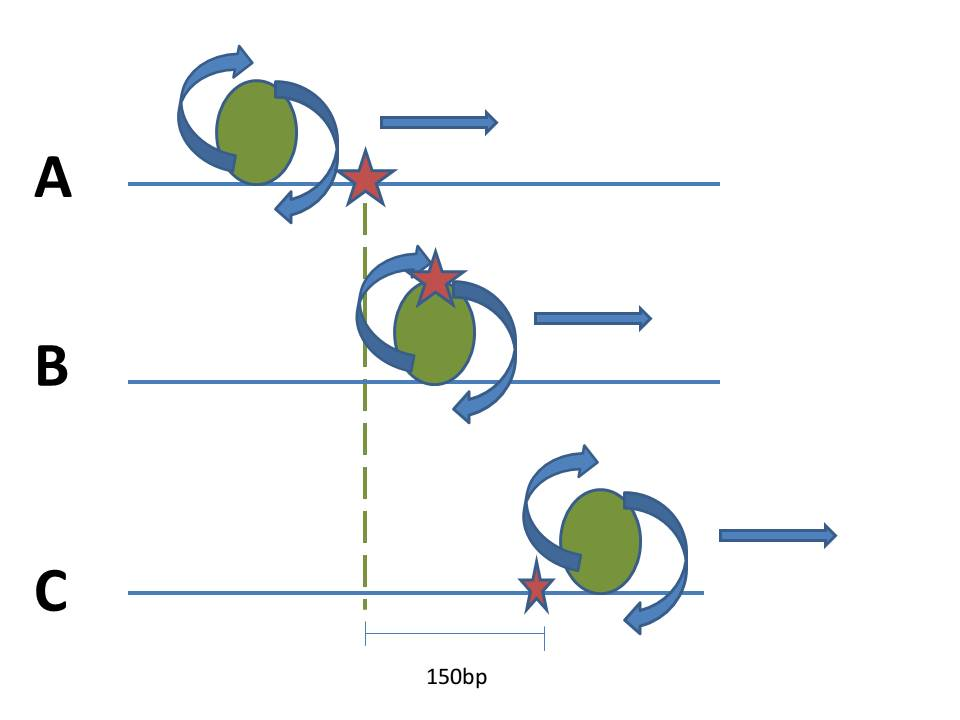
\includegraphics[width=0.7\linewidth]{histoneSlidingSingle}
	\caption{{Three time points during a displacement of damage site (red star) caused by histone rolling. The displacement of the damage site is equivalent to the length of DNA wrapped on a histone. A displacement is relative to some reference point, like the origin, and does not refer to an actual motion on the DNA}}
	\label{fig:histoneSlidingSingle}
	\end{figure}
		
	\begin{figure}
	\centering
	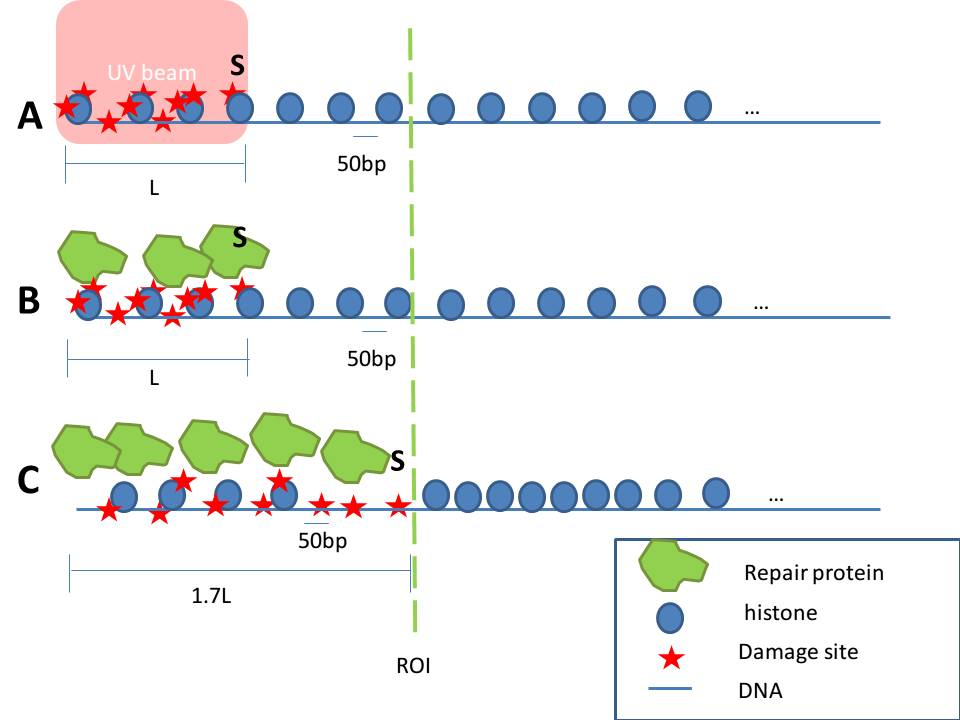
\includegraphics[width=0.7\linewidth]{histoneSlidingMulti}
	\caption{Expansion of the ROI due to nucleusome rolling. \textbf{A}. a UV beam (transparent red) damages DNA, with the point $S$ being the rightmost damage site \textbf{B}. Repair proteins (green polygons) are recruited to the damage site and start to expose the DNA in order the repair damages. \textbf{C}. Sliding the nucleosomes to the right in order to expose damage sites, translates the point $S$ to the right until $S$ reached $sqrt{3}L$. Repair proteins are present at the new location. The presence of repair proteins in $\sqrt{3}L$ indicates the ROI's boundary (vertical dashed green line). All DNA and histones to the right of $S$ are lost}
	\label{fig:histoneSlidingMulti}
	\end{figure}
	
	\section{2D model}
	
	
\end{document}